\documentclass{article}
\usepackage{graphicx} % Required for inserting images

\title{QuESt: Analysis for Regulators}
\date{}

\begin{document}

\maketitle

\section{Introduction}
QuESt: Analysis for Regulators (QAFR) is a lightweight tool designed to allow policymakers quick analysis of Energy Storage and renewable energy requirements for future generation buildouts. The core of the tool is a daily energy balance optimization problem that finds the minimum cost solution at the system level. QAFR is part of QuESt 2.0: Open Source Platform for Energy Storage Analytics. 

\section{Key Features}
QuESt: Analysis for Regulators has the following key features:

\begin{itemize}
    \item Determine minimum cost optimal requirements for Energy Storage, Wind, and PV at the system level. 
    \item Customize candidate Energy Storage devices by setting the round trip energy efficiency, annual degradation rate, end of life capacity, duration, and cycling requirements. 
    \item Set Renewable Portfolio Standard (RPS) targets throughout the time horizon of the study.
    \item Results dashboard highlighting key outputs of the analysis. 
\end{itemize}

\section{Data Requirements}

QuESt: Analysis for Regulators requires several pieces of data for simulation. Examples of necessary files can be found in the data directory including generation capacity targets, load profiles, and renewable profiles.

\begin{itemize}
    \item Projected system hourly load over the time horizon. 
    \item Hourly system level representative solar and wind profiles.
    \item Generation capacity targets.
    \item Estimated costs of solar, wind, and energy storage technologies.
\end{itemize}

\section{App Workflow}
To begin, load the QuESt: Analysis for Regulators app through the main QuESt page. Once complete click on the launch button which will take you to the landing page.

\begin{center}
    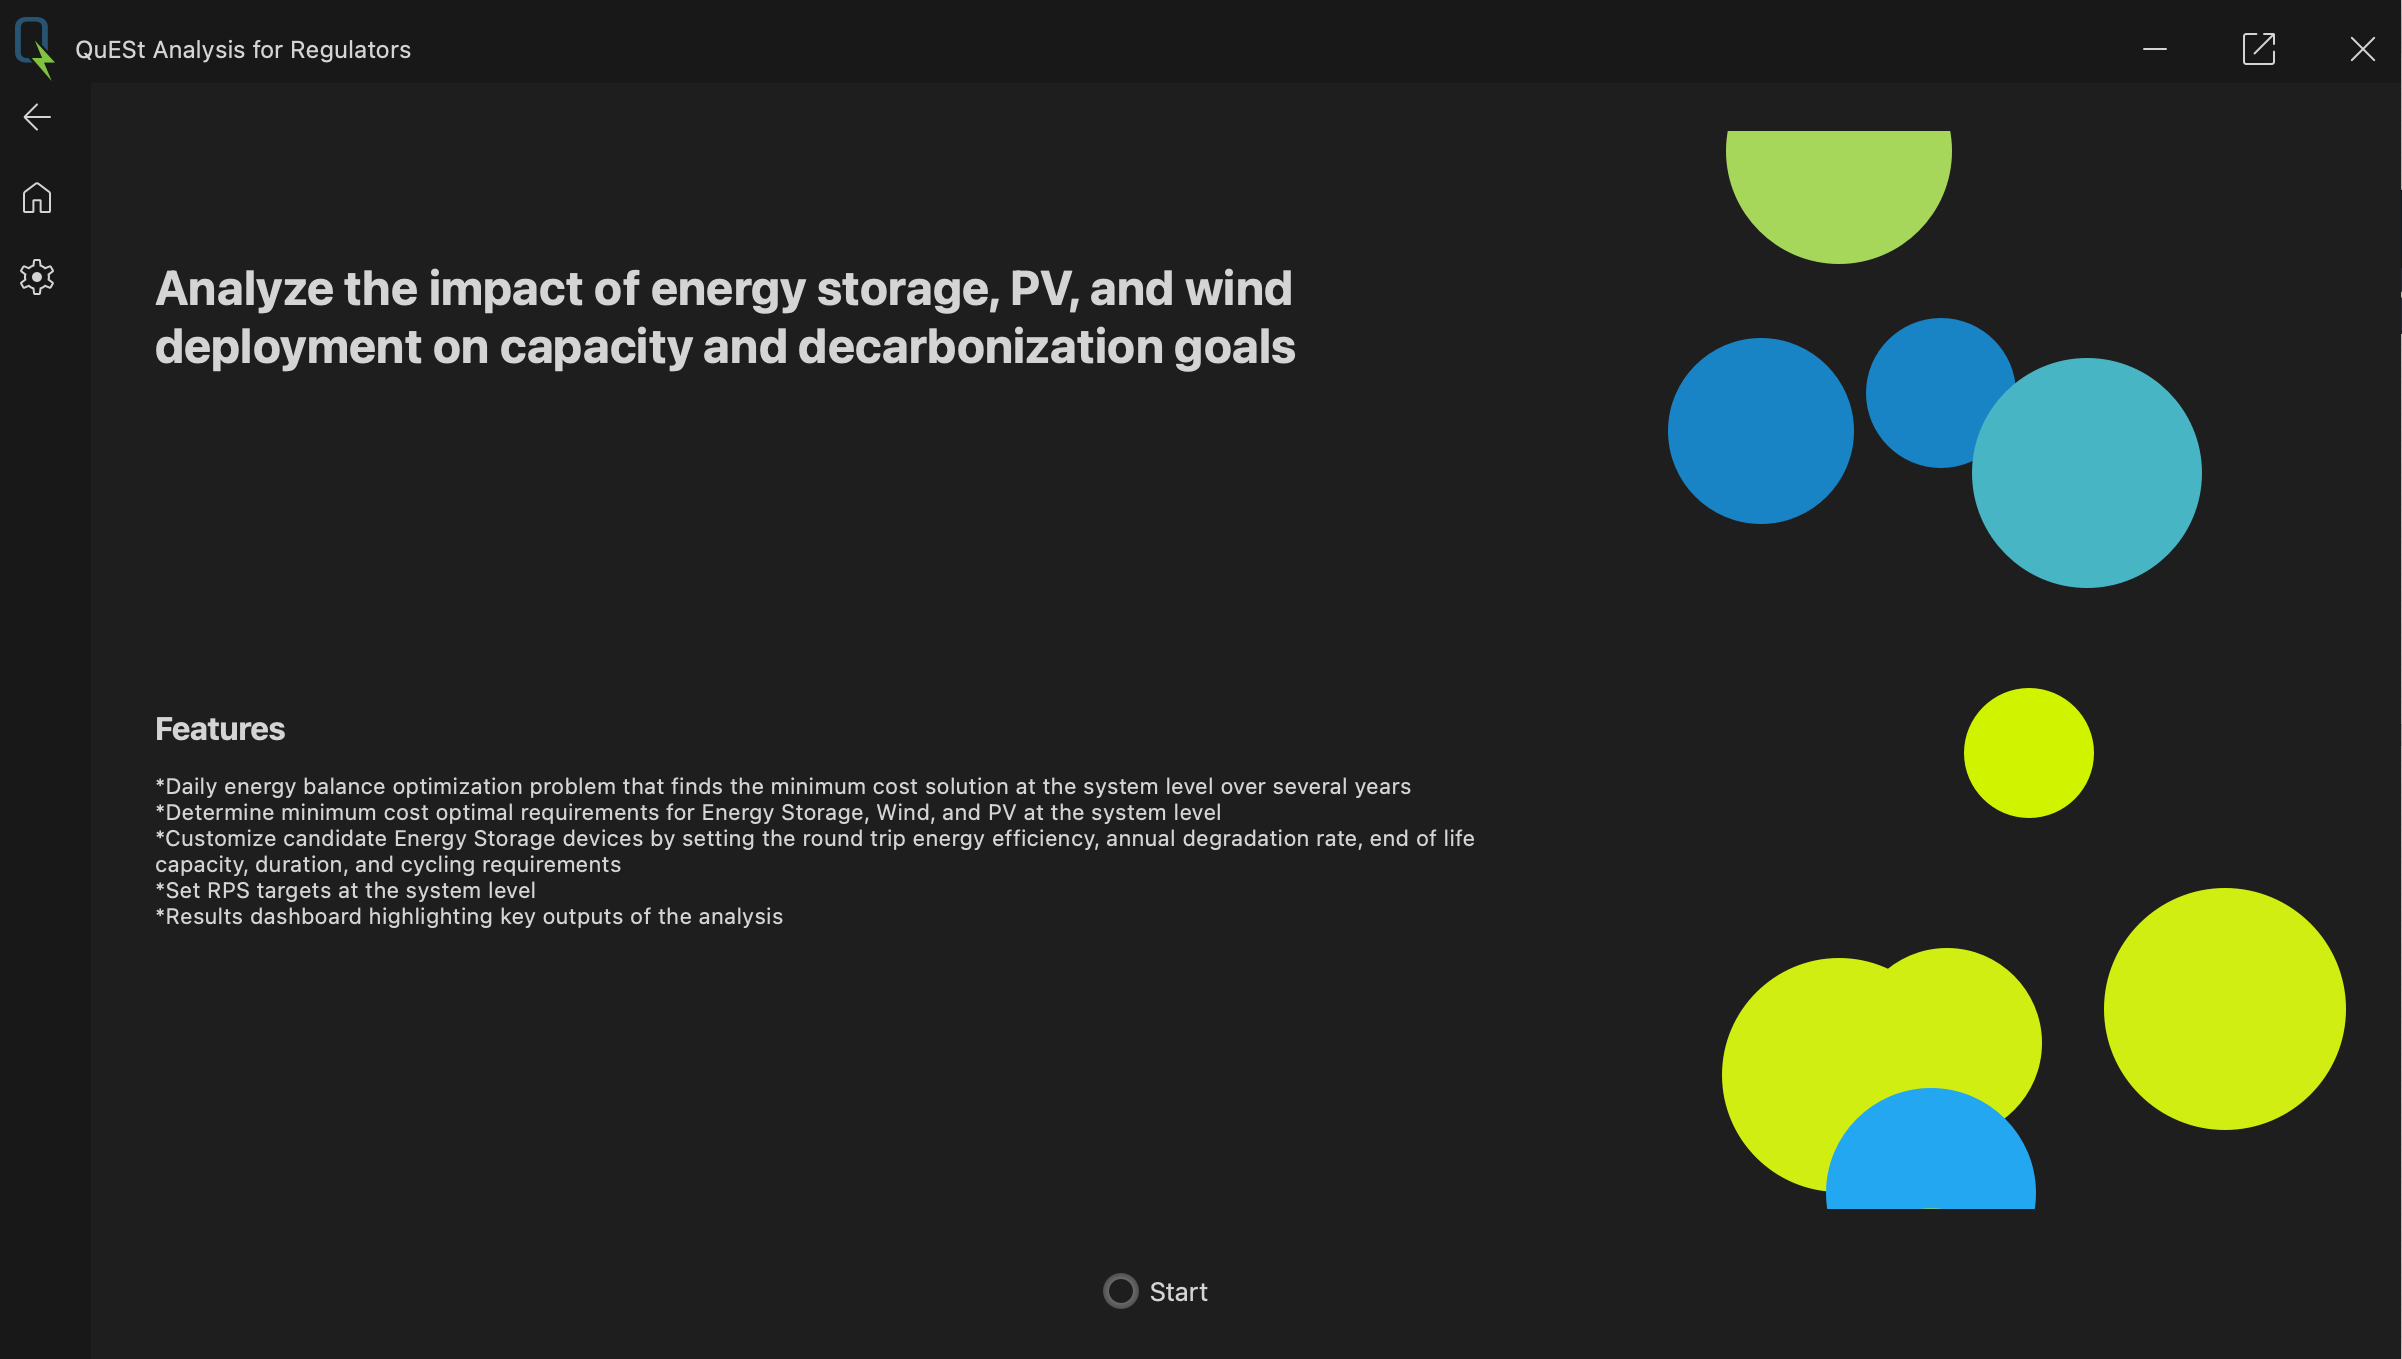
\includegraphics[width=0.8\linewidth]{pics/landing_page.png}
\end{center}
The landing page lists details and features of the app. Click next to open the load, insolation, and wind power file upload page. 

\begin{center}
    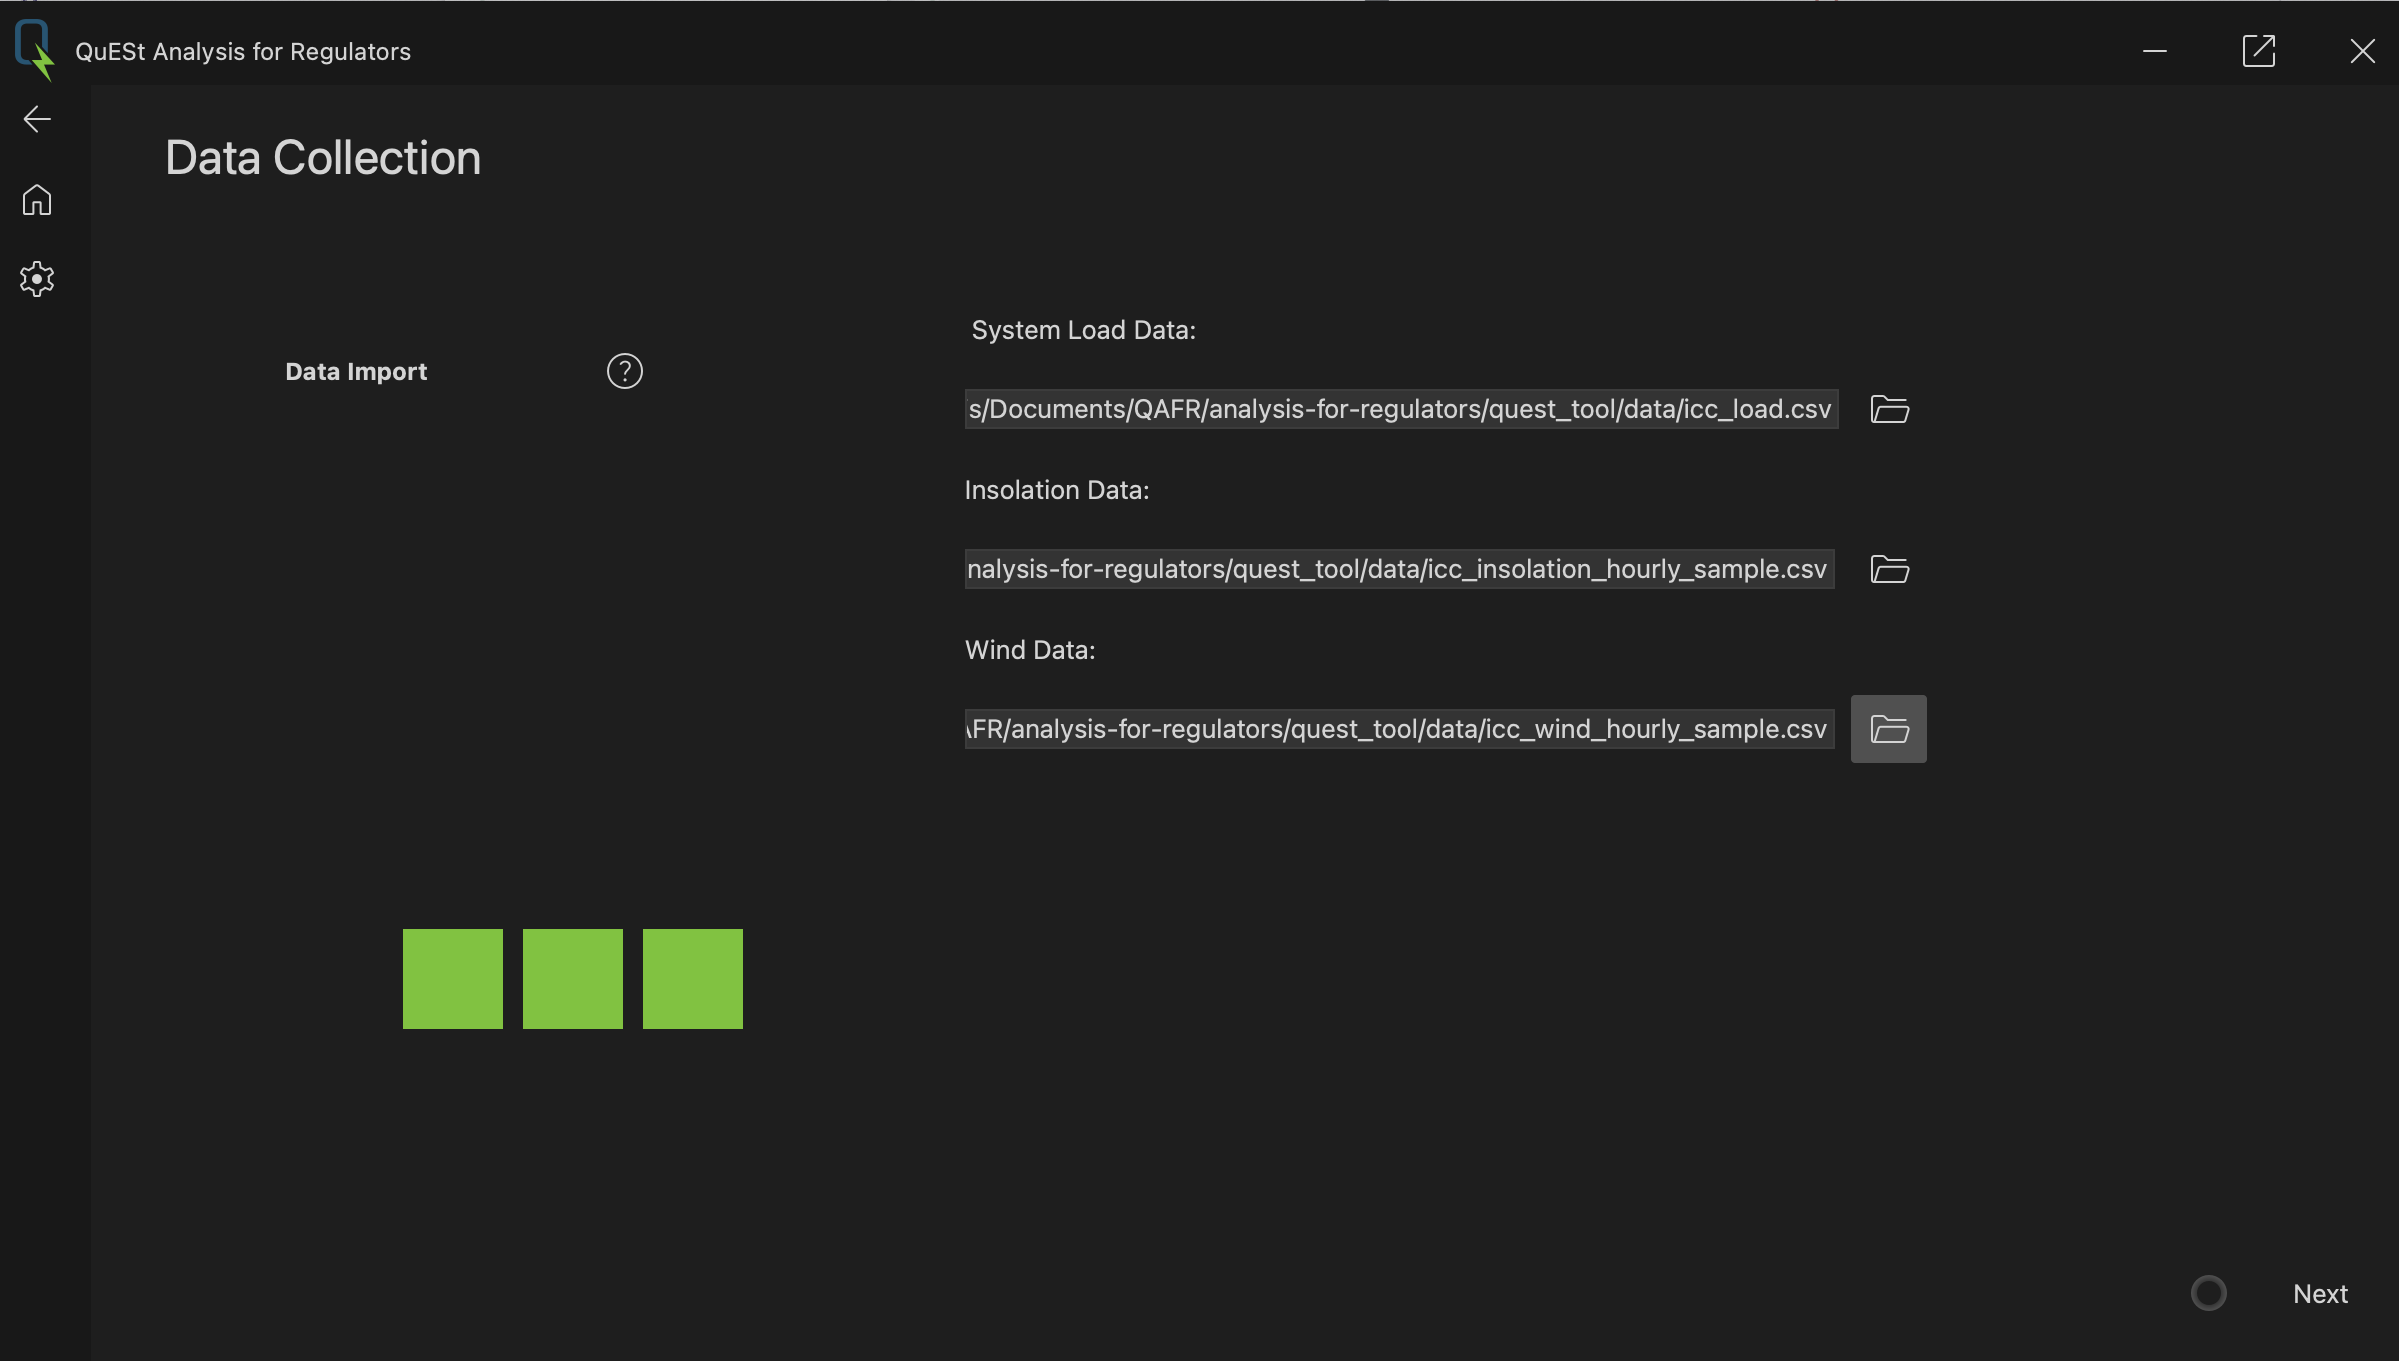
\includegraphics[width=0.8\linewidth]{pics/file_page.png}
\end{center}
Click on the file browser buttons to find and open the load profile, insolation profile, and wind profile of the desired system. Once they are selected click on the next button to move on to the following page.

\begin{center}
    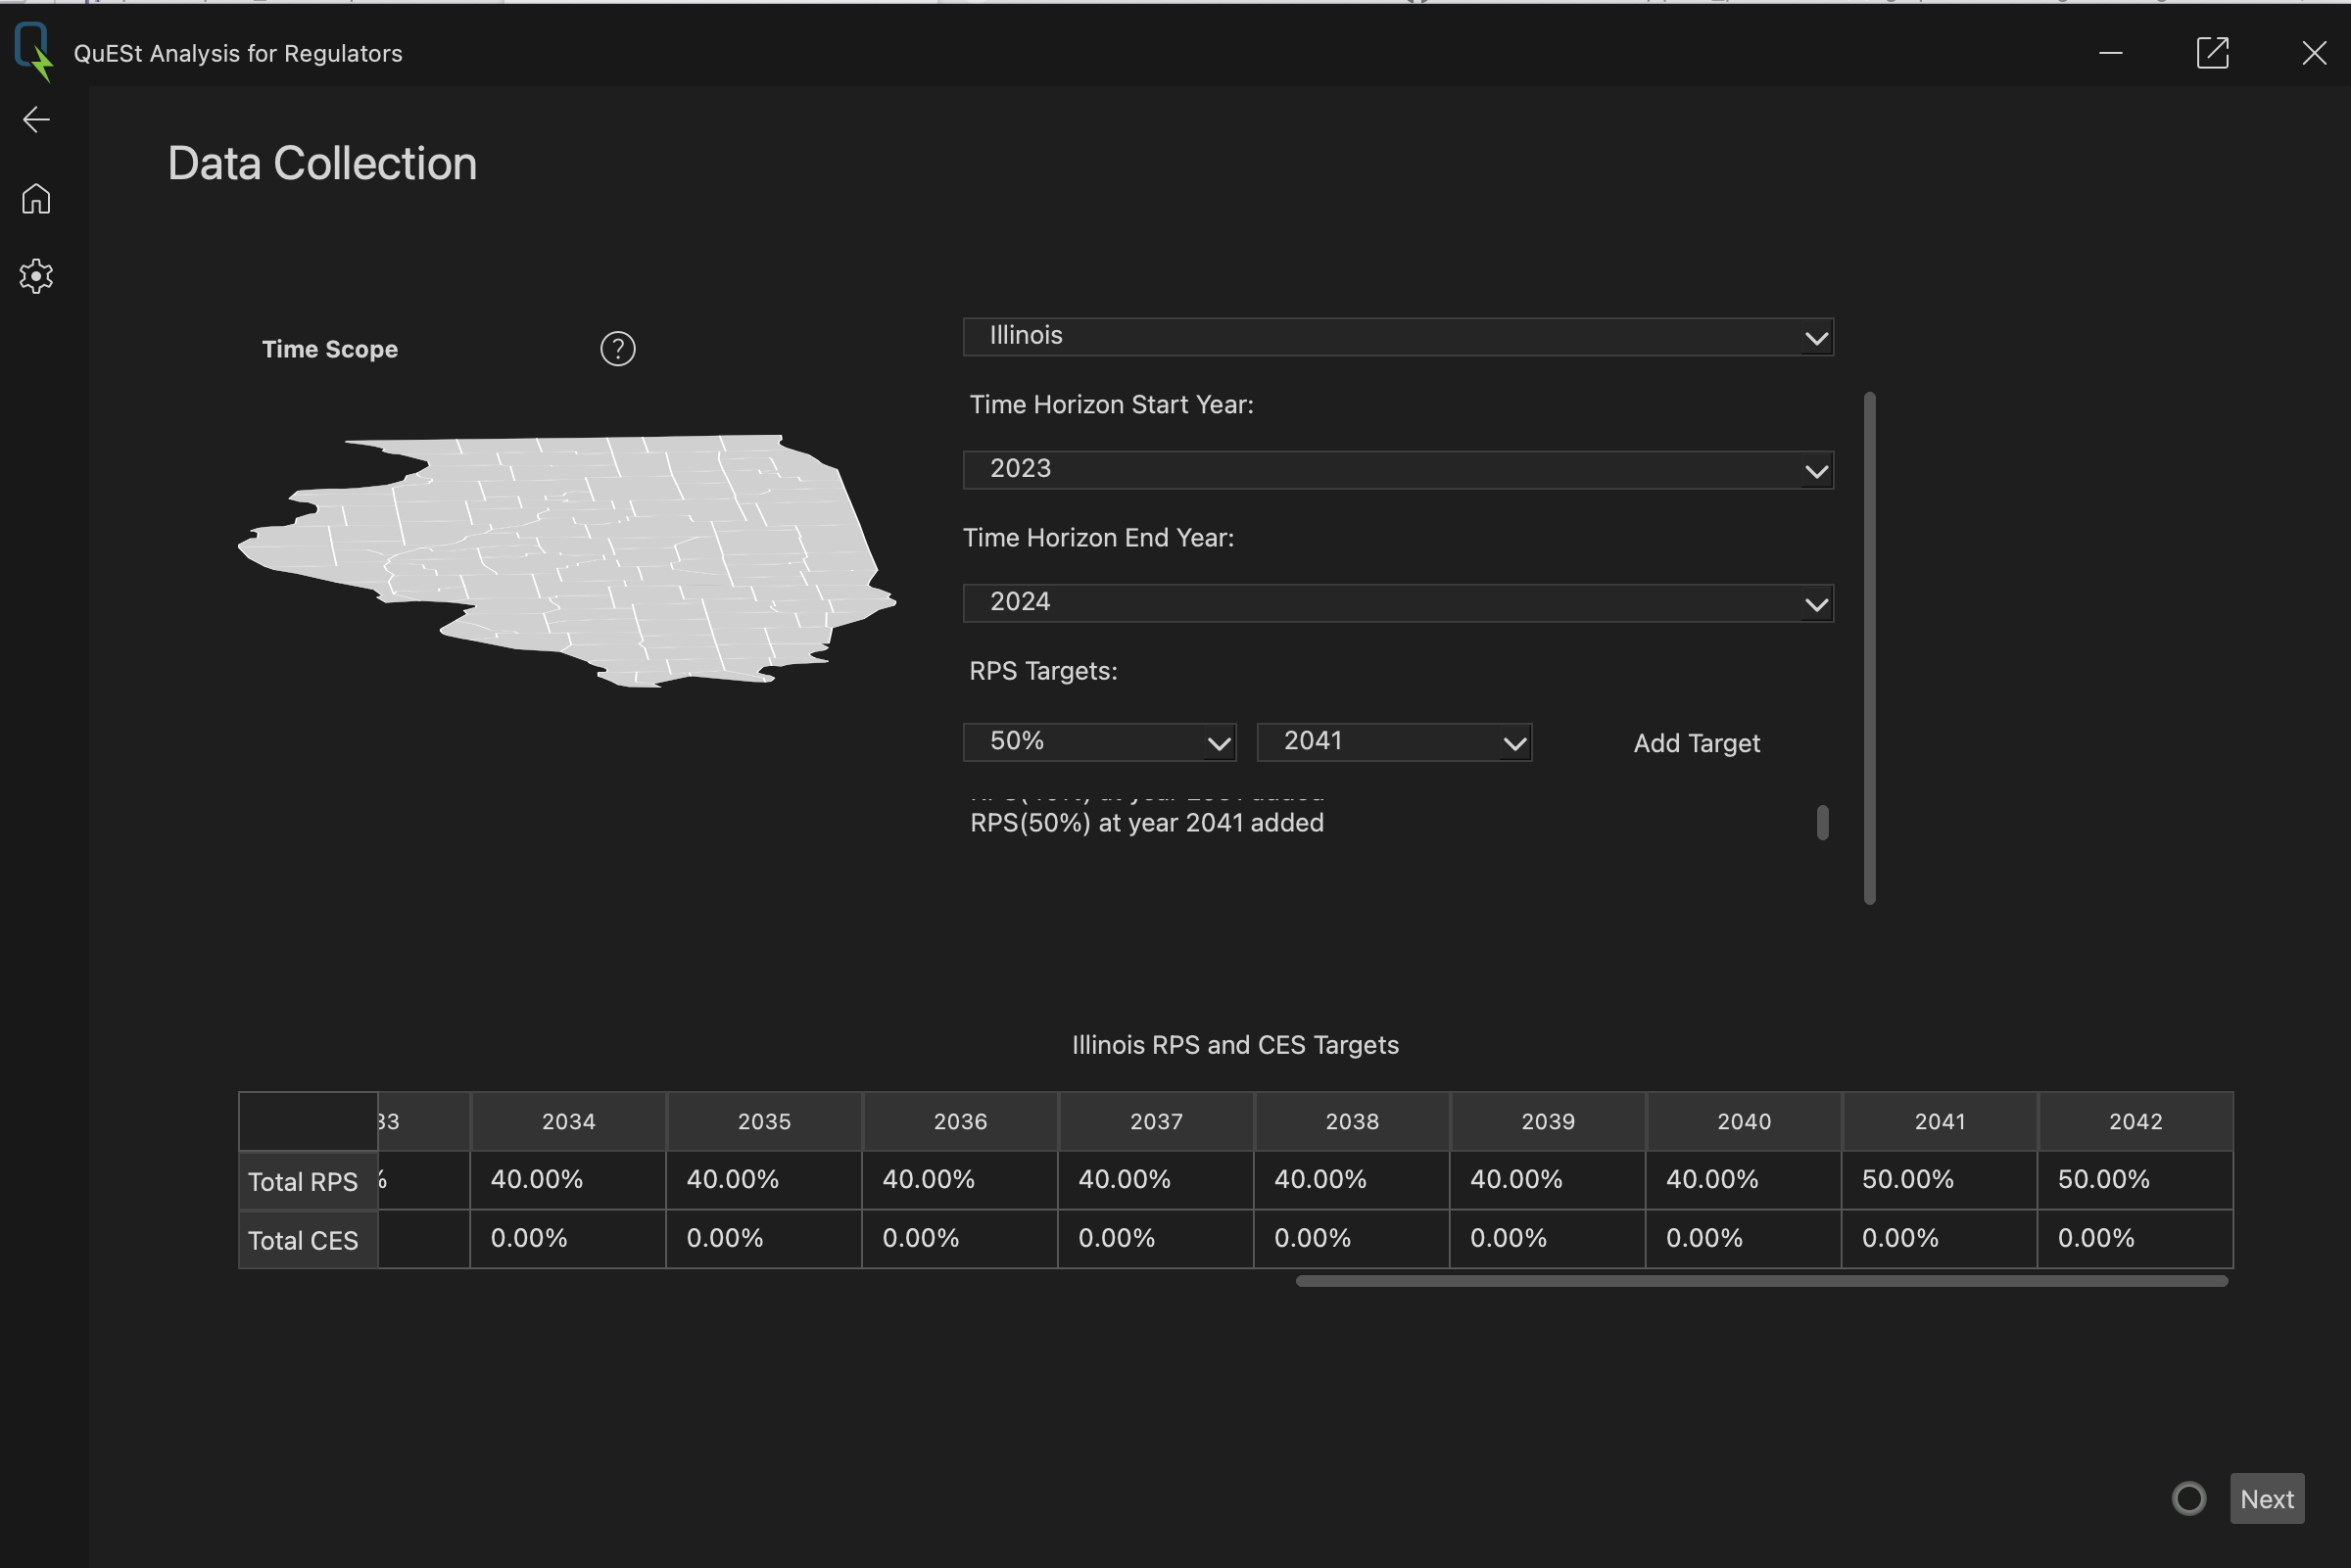
\includegraphics[width=0.8\linewidth]{pics/time_horizon.png}
\end{center}
On the time scope page the time horizon and RPS targets will be set. The start and end years can be selected from the years given in the load data uploaded on the previous page. Upon selecting a state, the RPS and CES targets will populated in the lower table which represent values available from Berkely Lab Energy and Markets Policy U.S. State Renewables Portfolio and Clean Energy Standards 2024 Update which can be accessed at  https://emp.lbl.gov/publications/us-state-renewables-portfolio-clean-0. RPS targets may then be set using the values provided in the table or more aggressive or lenient targets may be set to compare to the current policies.

\begin{center}
    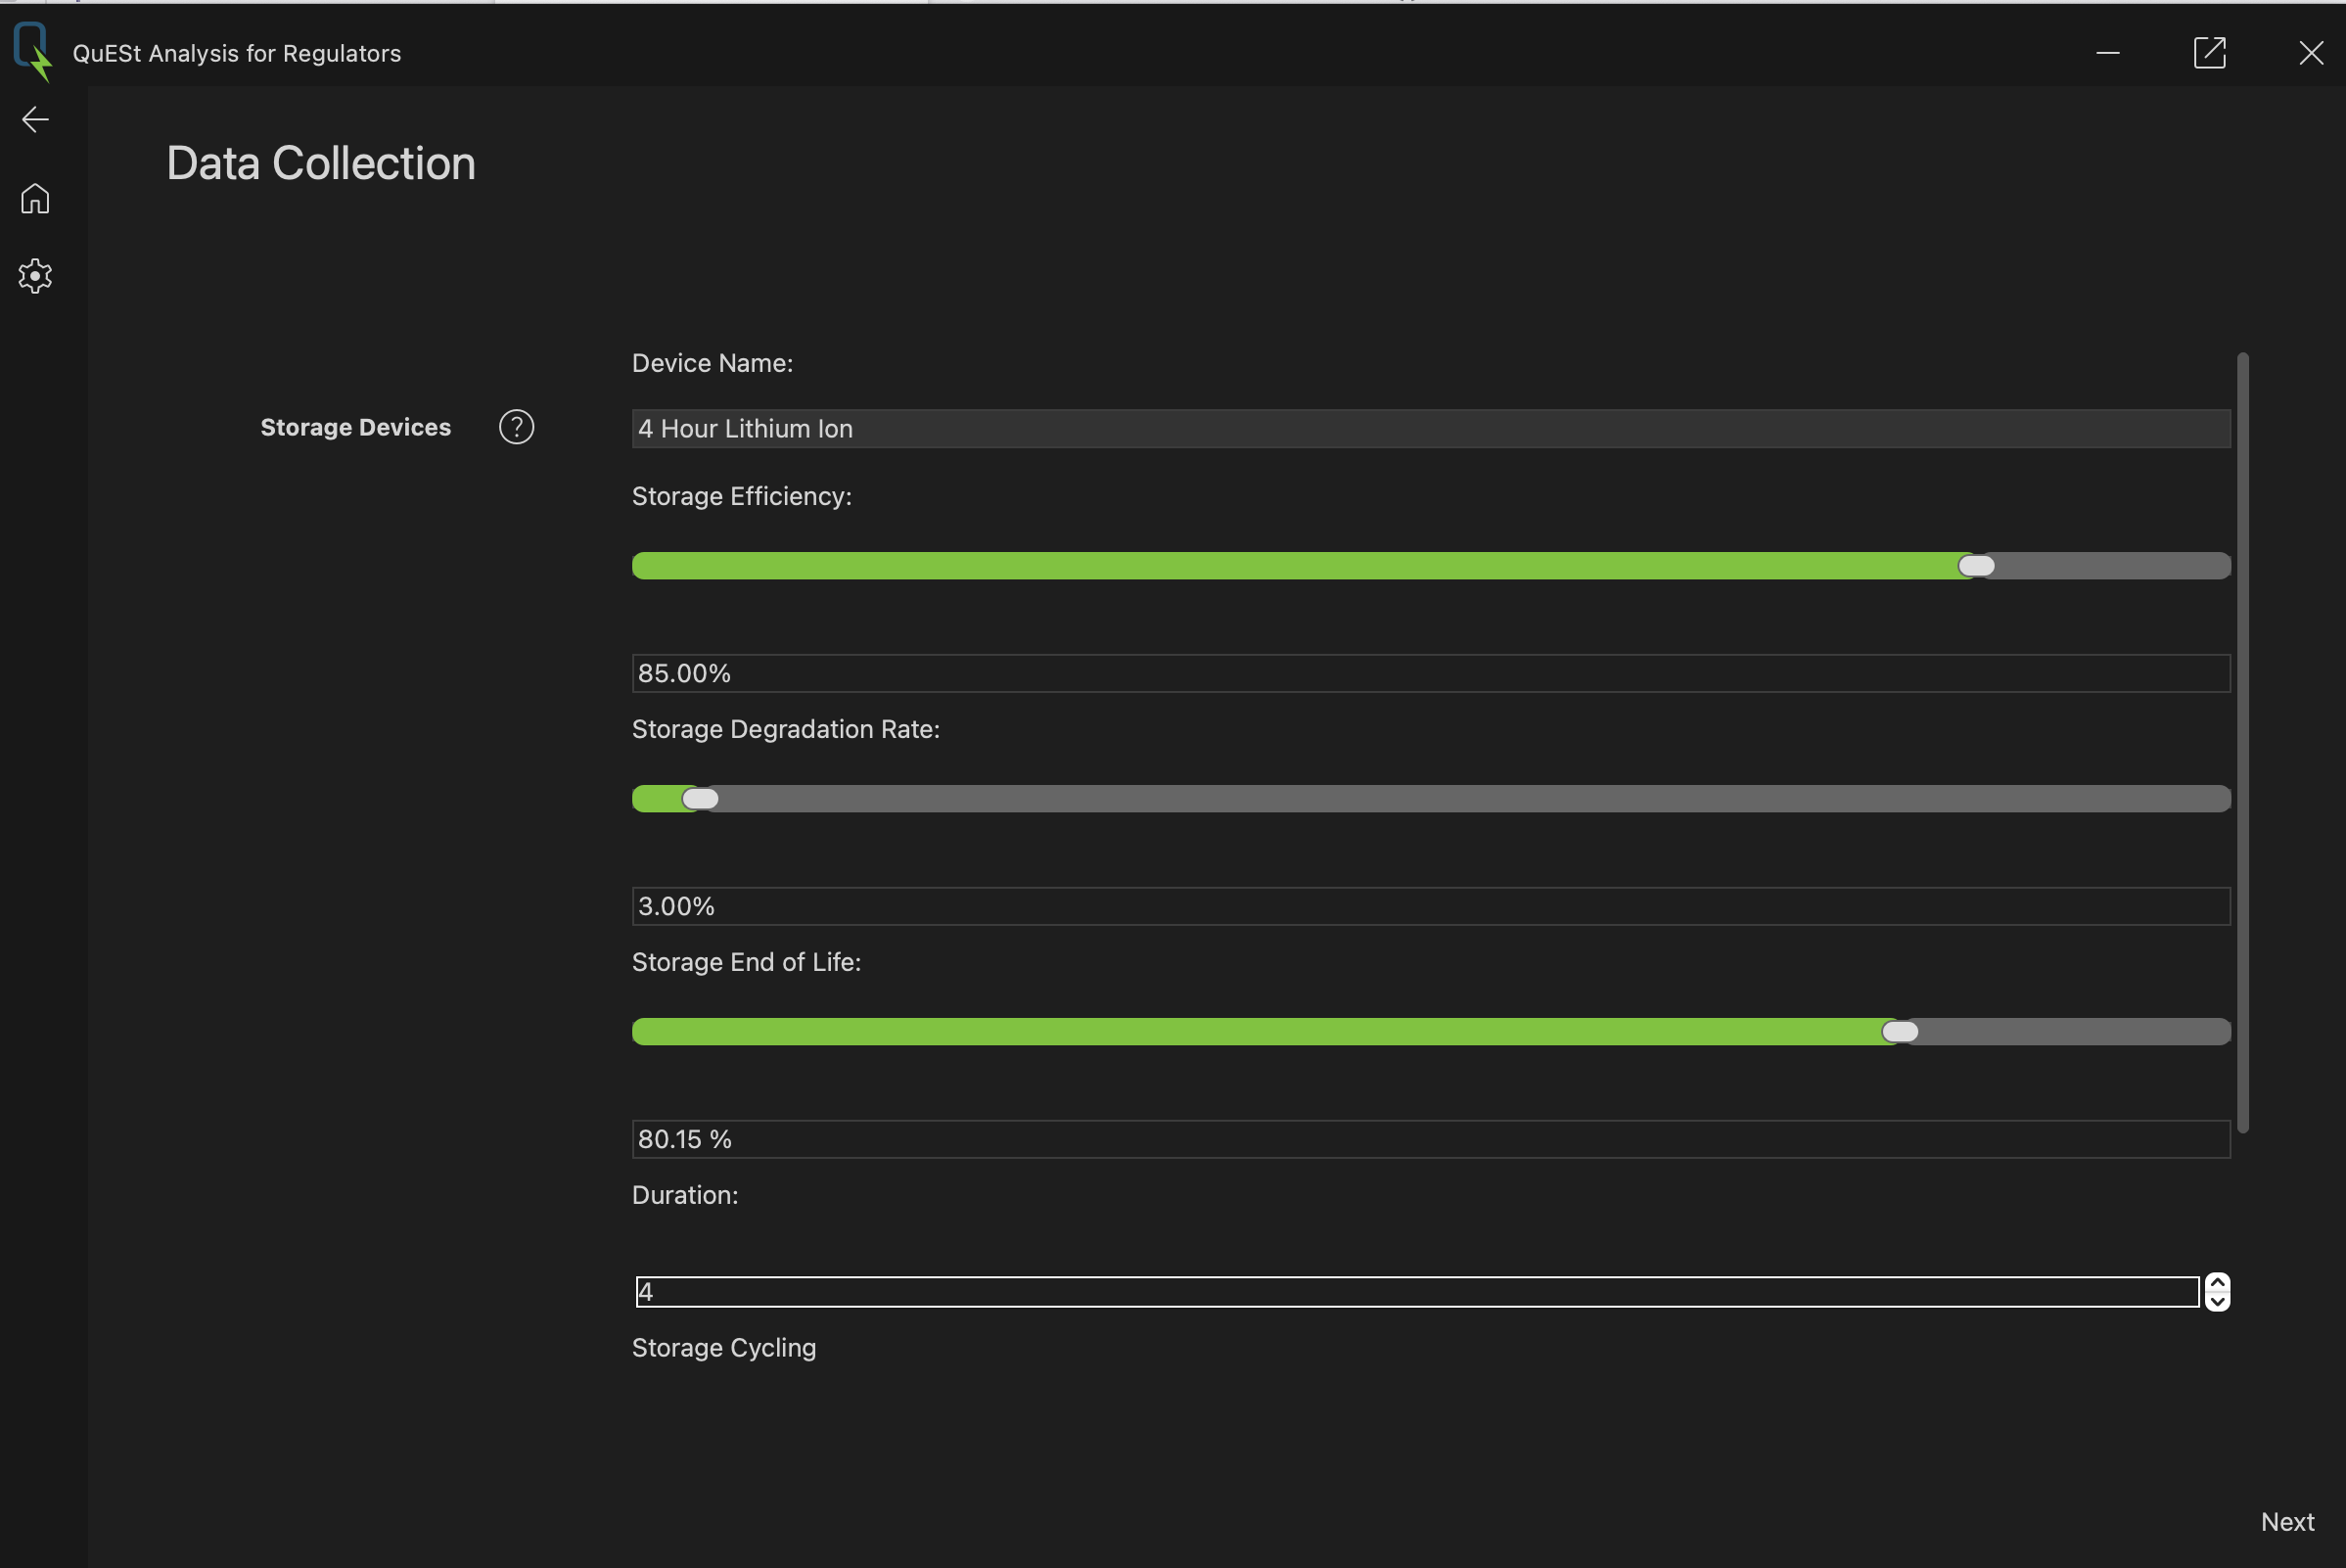
\includegraphics[width=0.8\linewidth]{pics/battery.png}
\end{center}
The next page custom ES devices may be created. Round trip efficiency, annual degradation rate, device end of life capacity percentage, duration, and cycling schedule may be specified.  

\begin{center}
    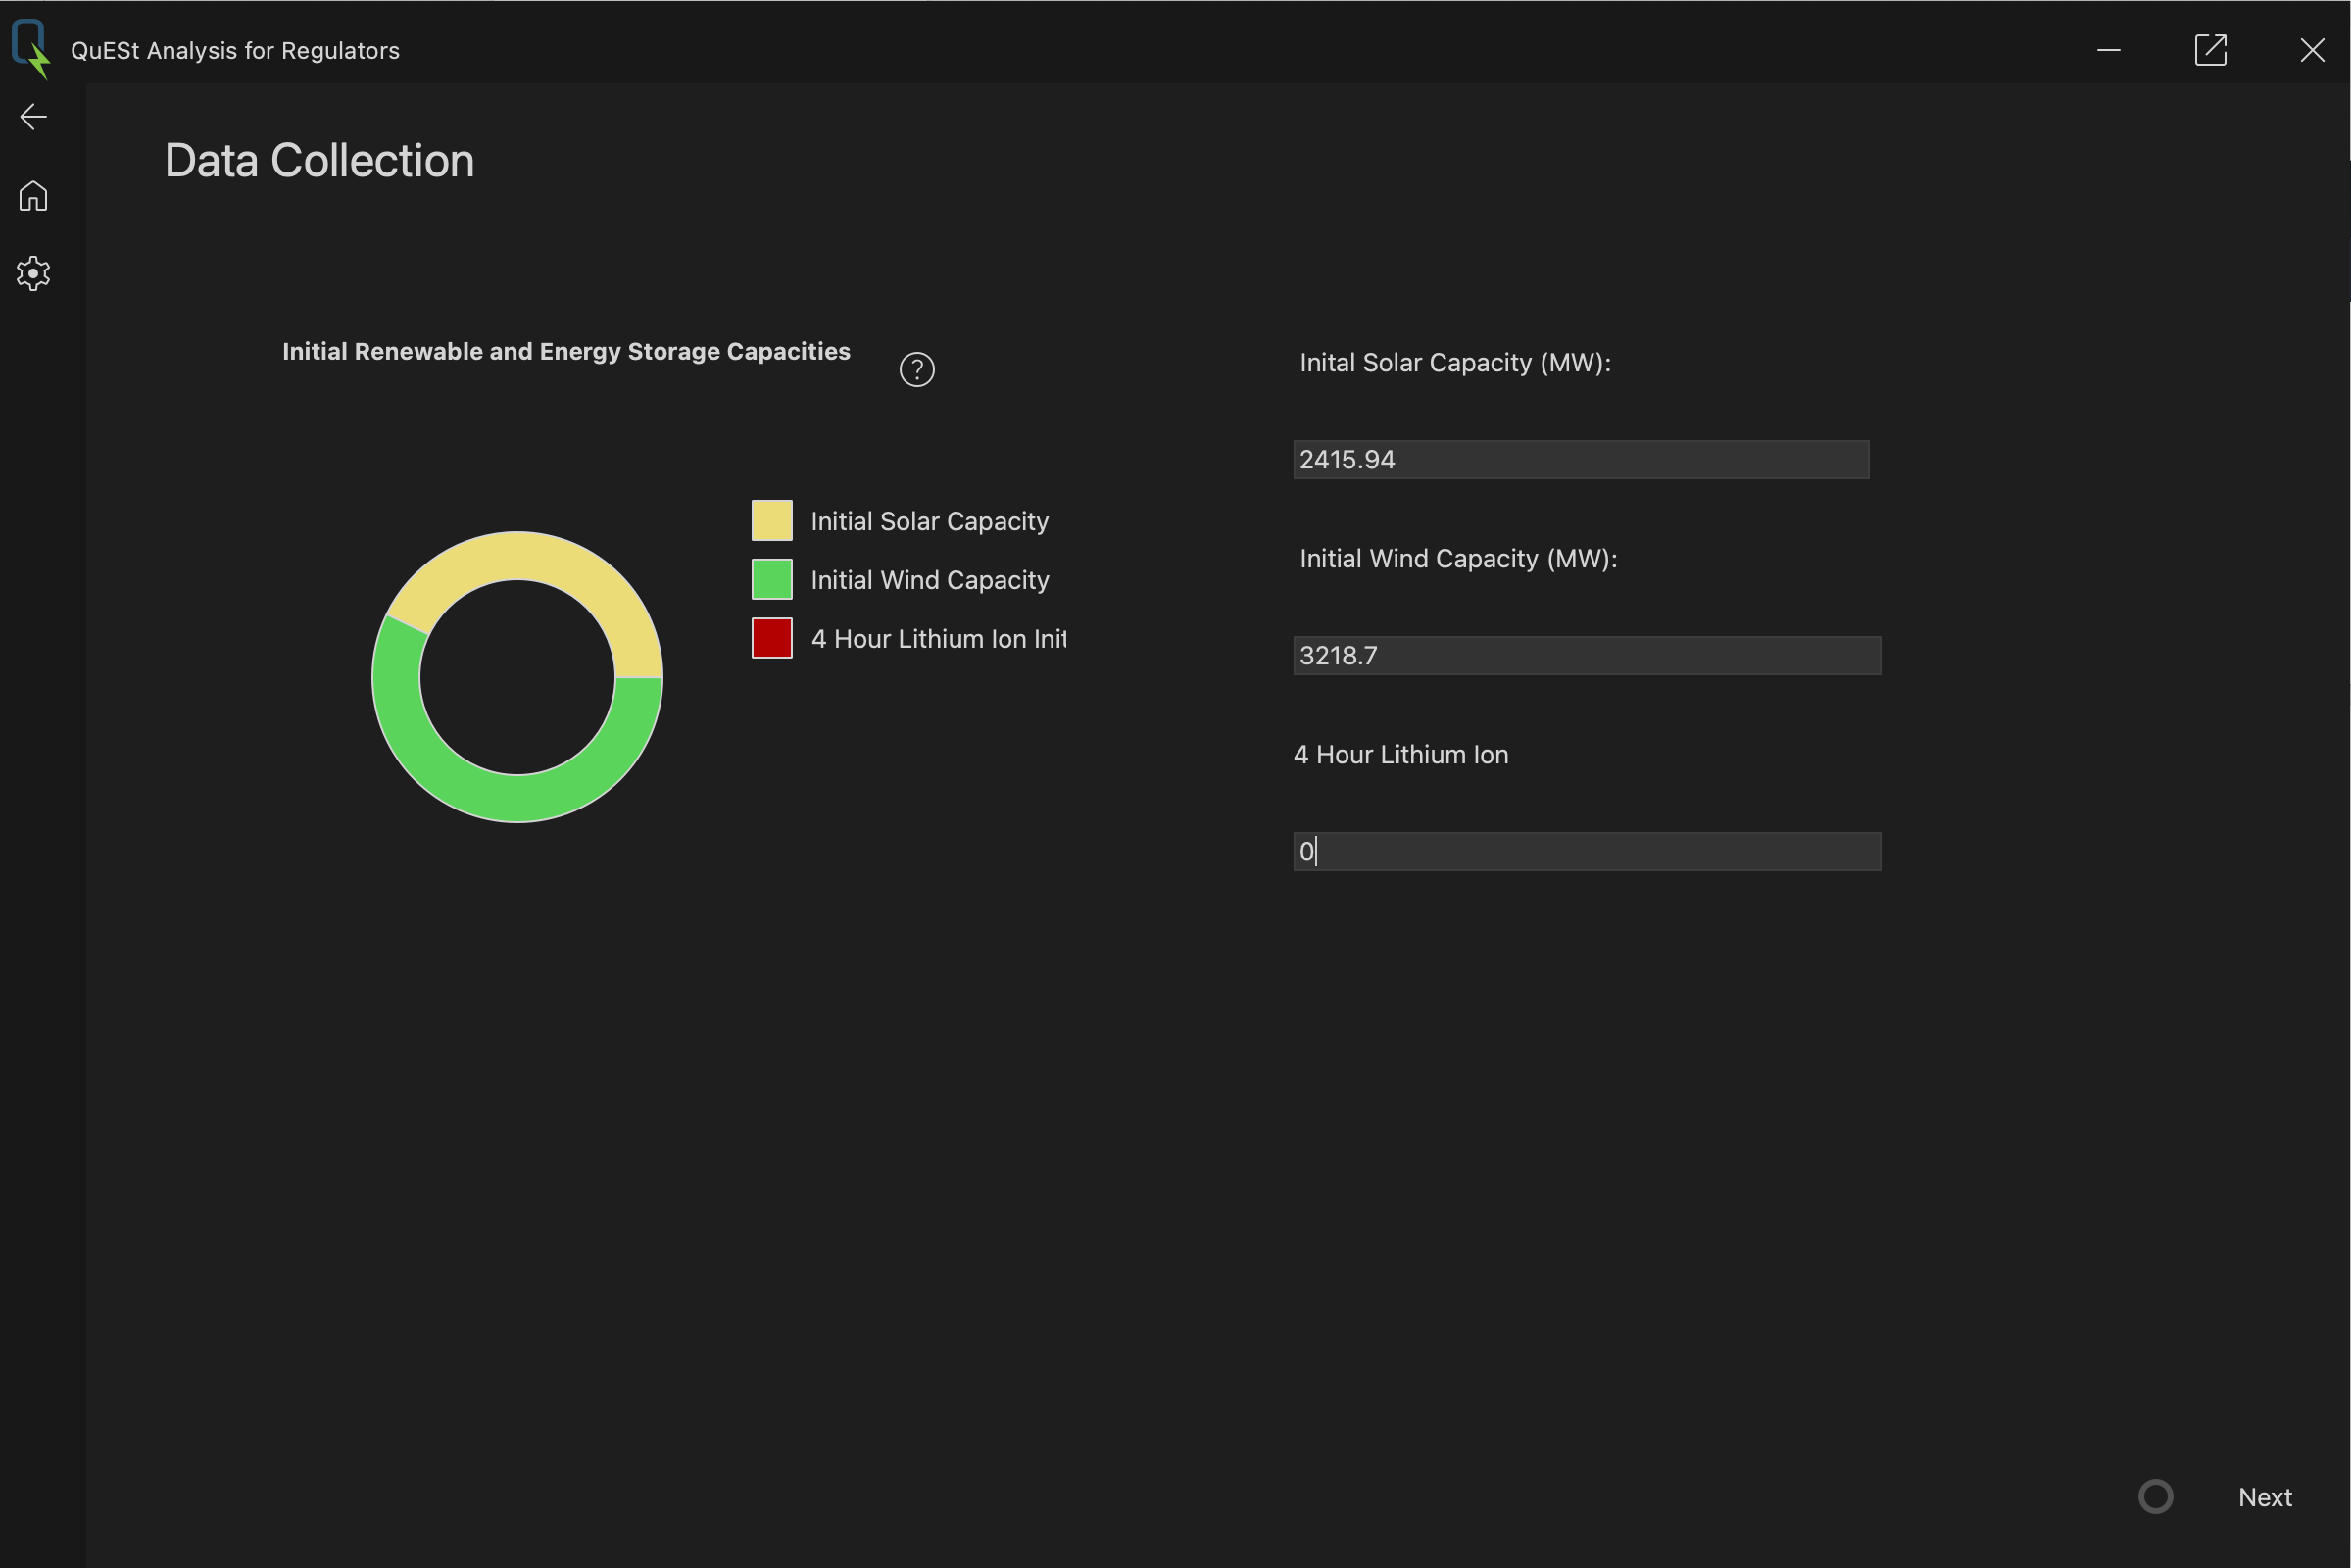
\includegraphics[width=0.8\linewidth]{pics/init_caps.png}
\end{center}
Following the ES page, initial capacities of each potential investment device will be set. This will be the amount of each technology currently available on the system. If there is none, set the device initial capacity to 0.

\begin{center}
    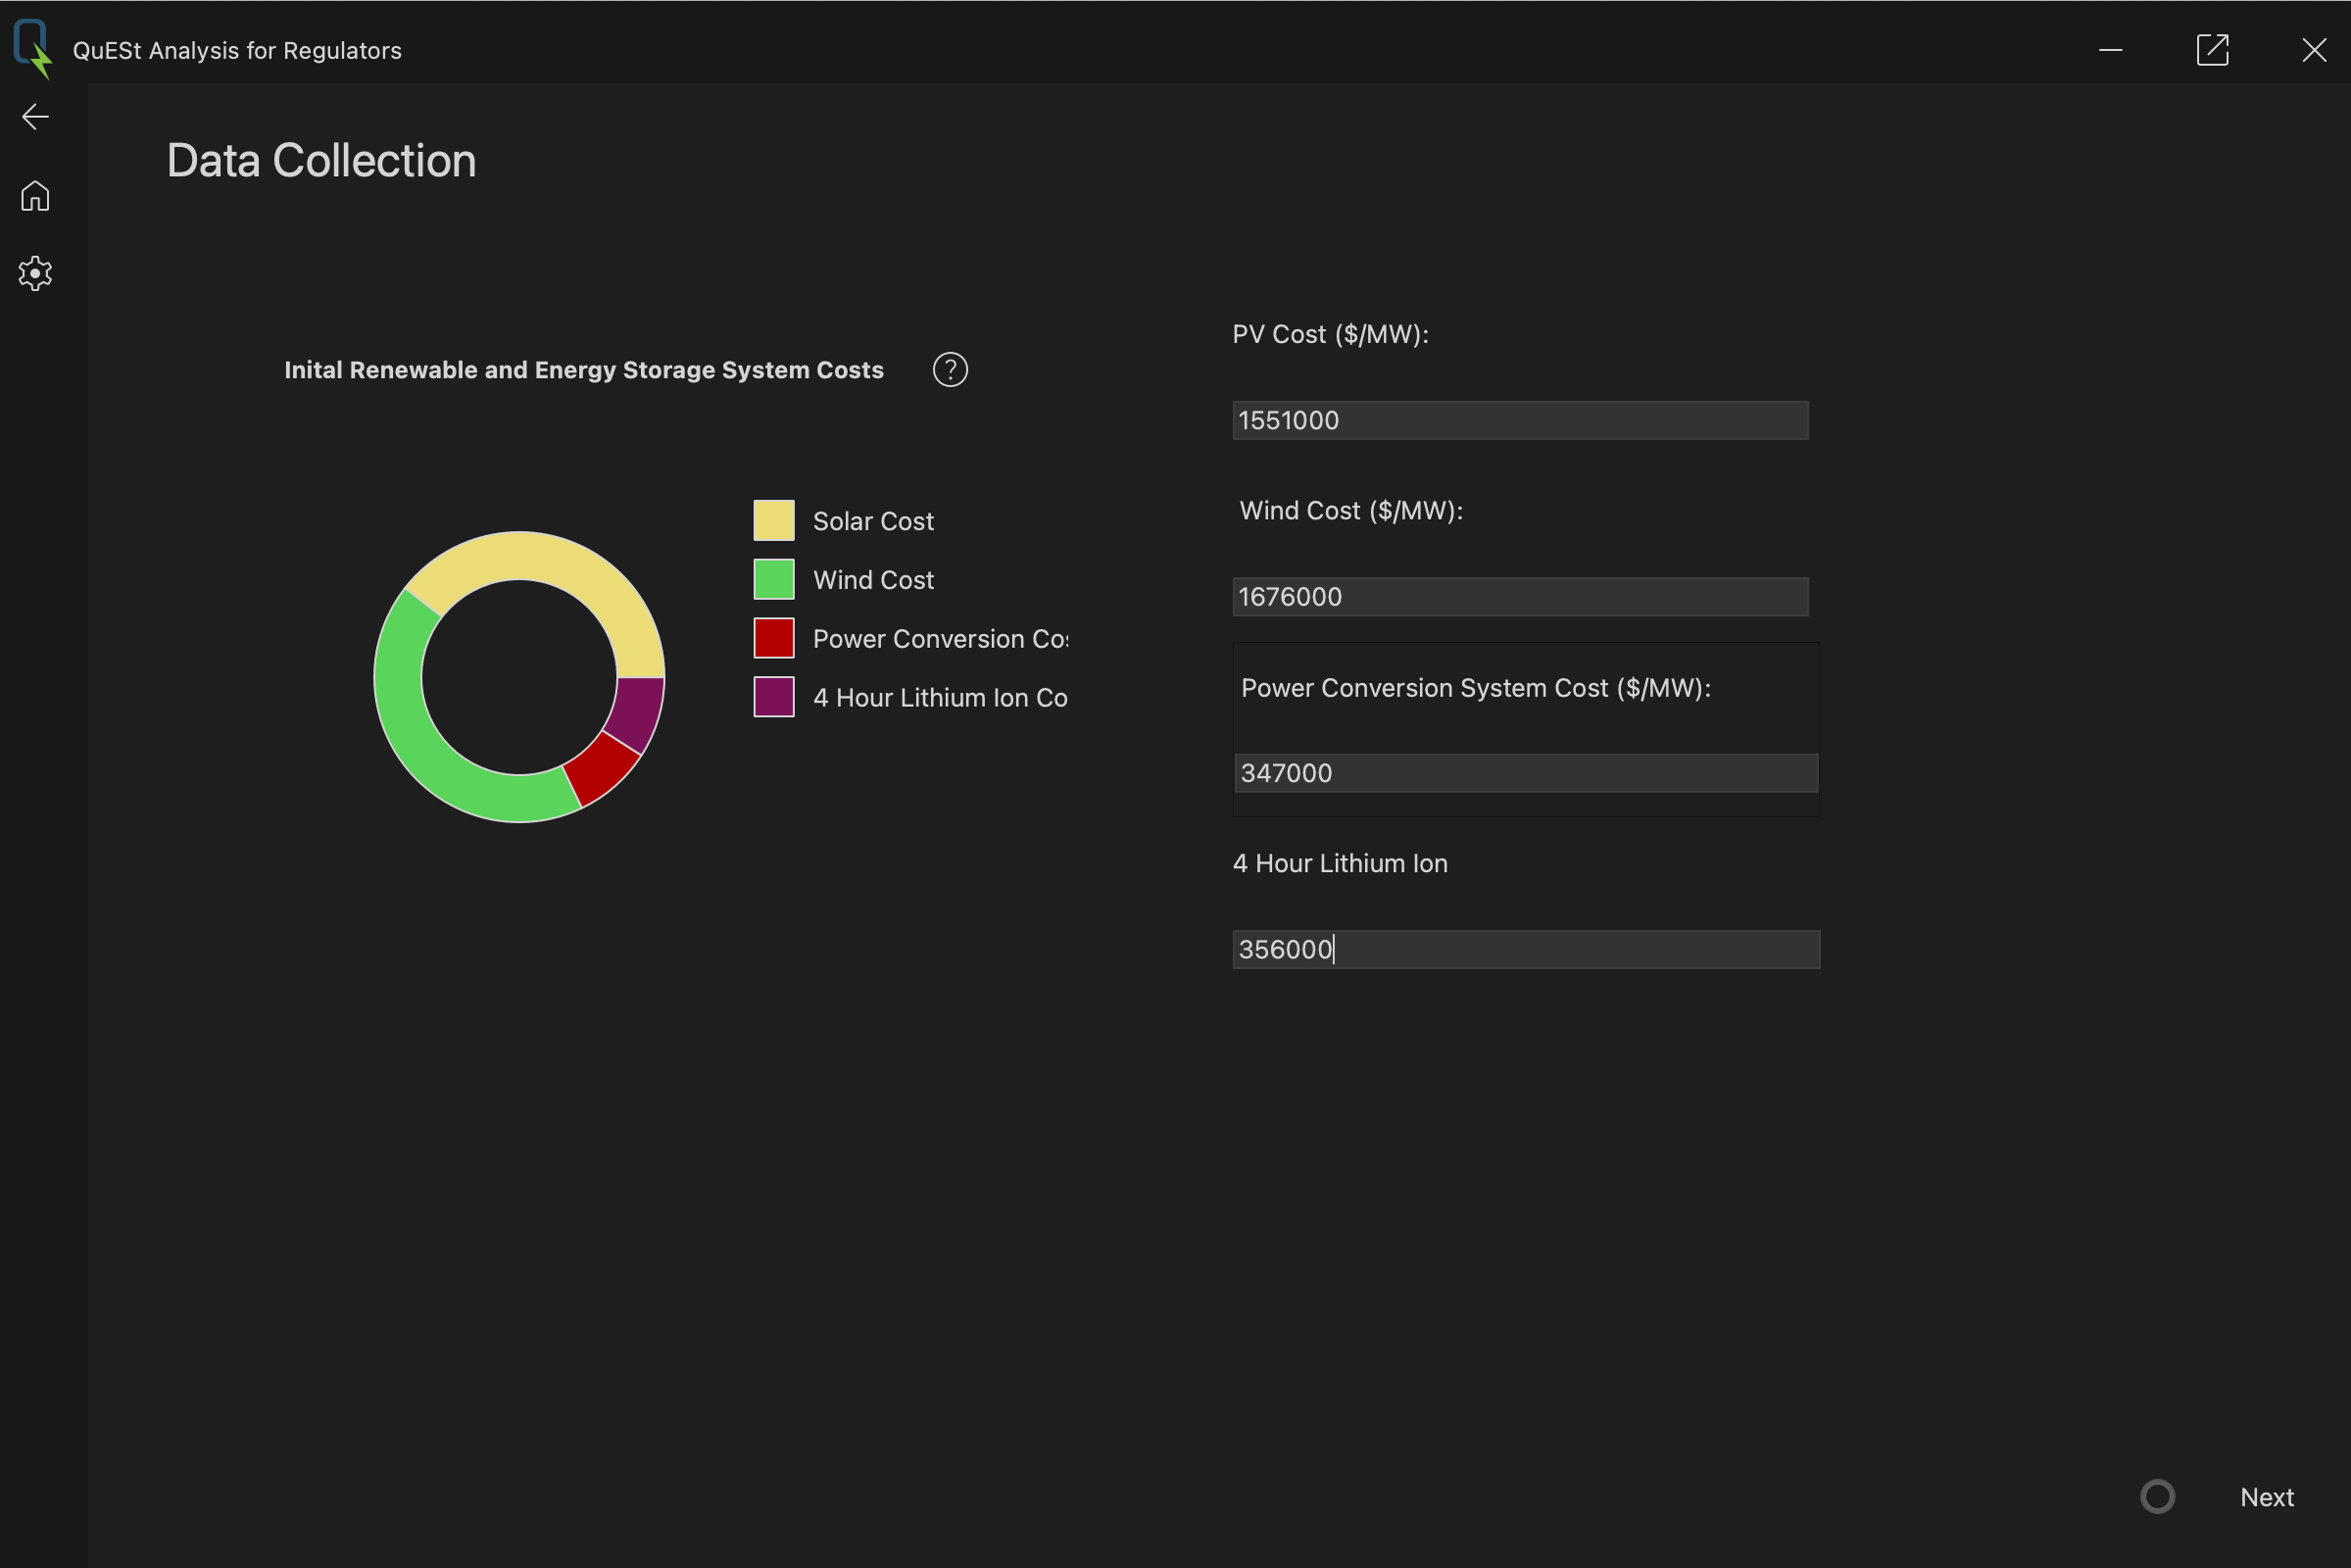
\includegraphics[width=0.8\linewidth]{pics/cap_cost.png}
\end{center}
Similarly, on the next page the initial capital costs of each potential investment device will be set. The costs are built with an annual 2.5\% discount rate. 

\begin{center}
    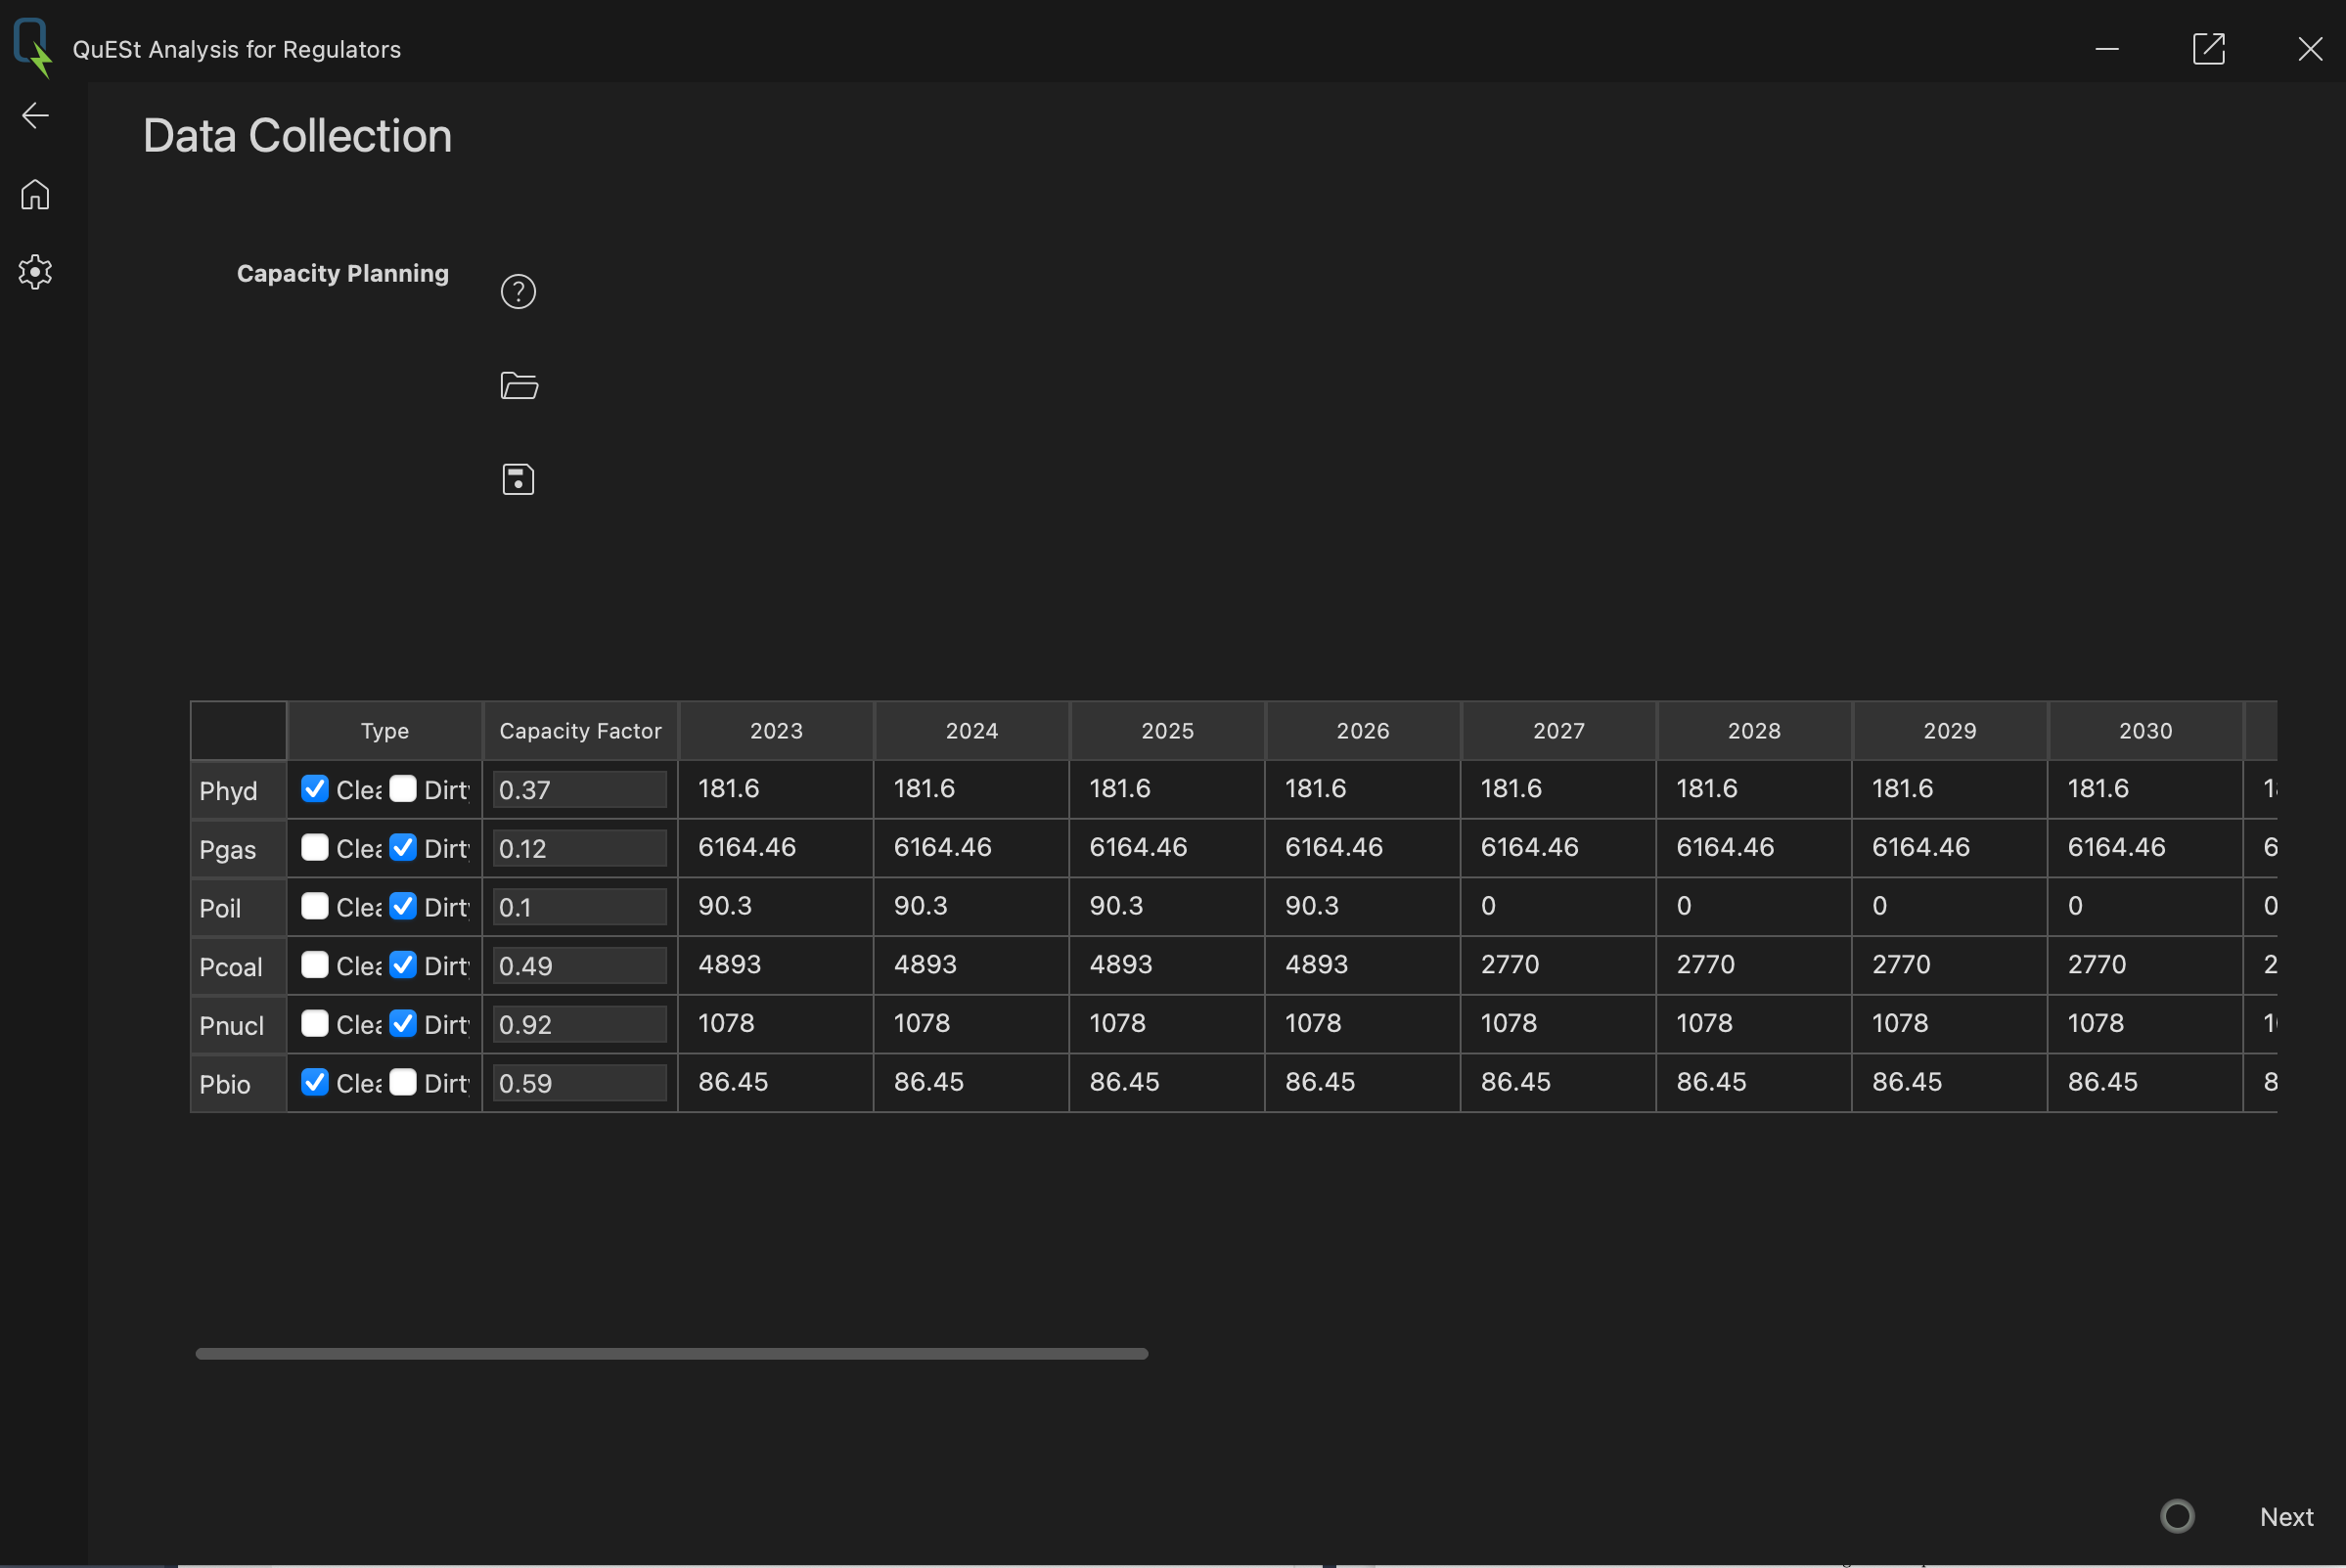
\includegraphics[width=0.8\linewidth]{pics/gen_caps.png}
\end{center}
Upon clicking the next button, the system generation targets will display. Open the file browser to load the system generator target table. This table should display target generator capacity of various technologies over the time horizon. The first two columns will also indicate whether the technology is considered to be a clean energy source or a dirty energy source, and the capacity factor of each technology. If changes are made to the initial values, the new table may be saved by clicking on the file save button. When ready, clicking next will begin the simulation.

\begin{center}
    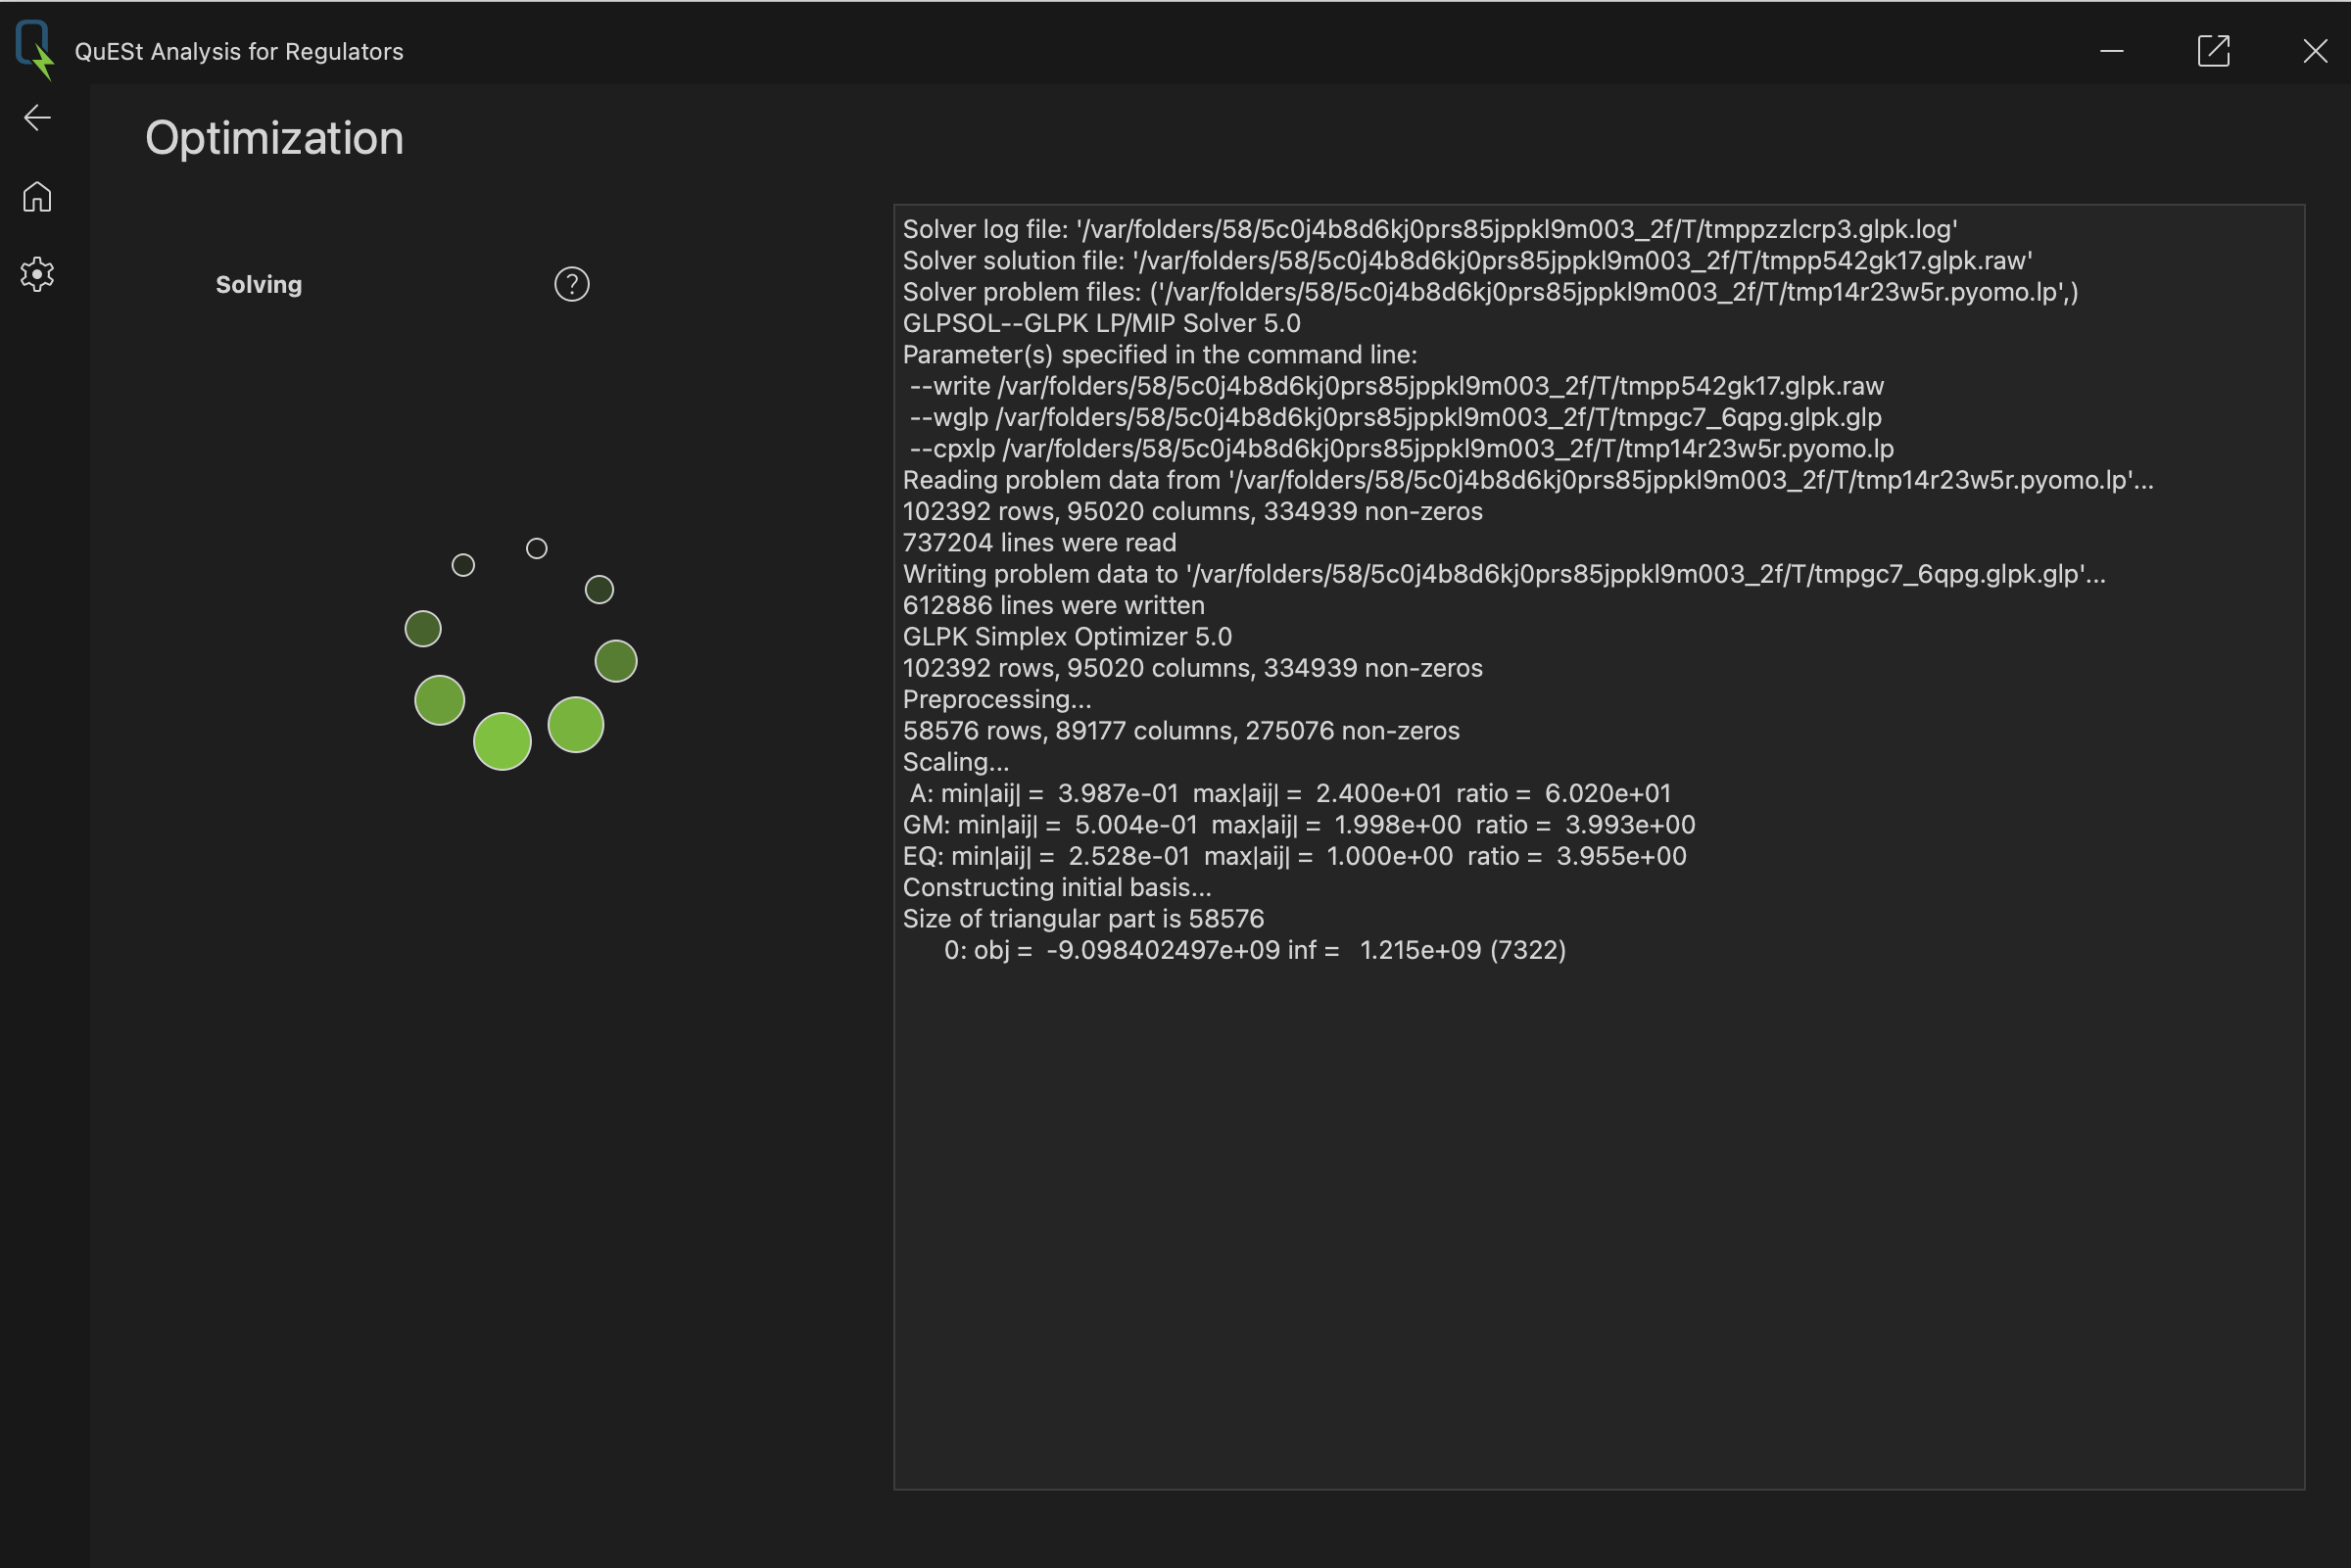
\includegraphics[width=0.8\linewidth]{pics/opt.png}
\end{center}
While the simulation is running, the optimization dashboard will display the progress of the simulation. Upon solving the results dashboard will populate.

The results dashboard contains the results of the analysis. The central plot contains several variables of interest including yearly investements, yearly capacities, seasonal energy consumption, etc. A pie chart also displays the generation mix by year. At the bottom of the page, a table displays the investments in solar, wind, and energy storage devices needed to achieve each RPS target set at the beginning. Below, the results of running the analysis for the state of Illinois based on the data collected from the MISO futures report found at https://www.misoenergy.org/planning/futures-development/.

Provided in the data folder of the tool are capacity targets and load profiles for each of the three future scenarios for load zone four of MISO corresponding to Illinois region. Additionally, a representative wind and solar profile for the state generated from data collected via NREL's wind and solar API are provided. In each following case, a four hour lithium ion battery is available for buildout with 85\% round trip efficiency, 3\% annual degradation rate, end of life at 80\% of capacity degradation, and weekly cycling schedule. The capital costs of this battery are taken from NREL's ATB at 347,000 \$/MW and 356,000 \$/MWh. There is assumed to be no energy storage currently on the system. The cost of wind and solar per MW are provided as default values, also gathered from NREL's ATB. RPS targets are set at 40\% in the year 2031 and 50\% in the year 2041.
\begin{center}
    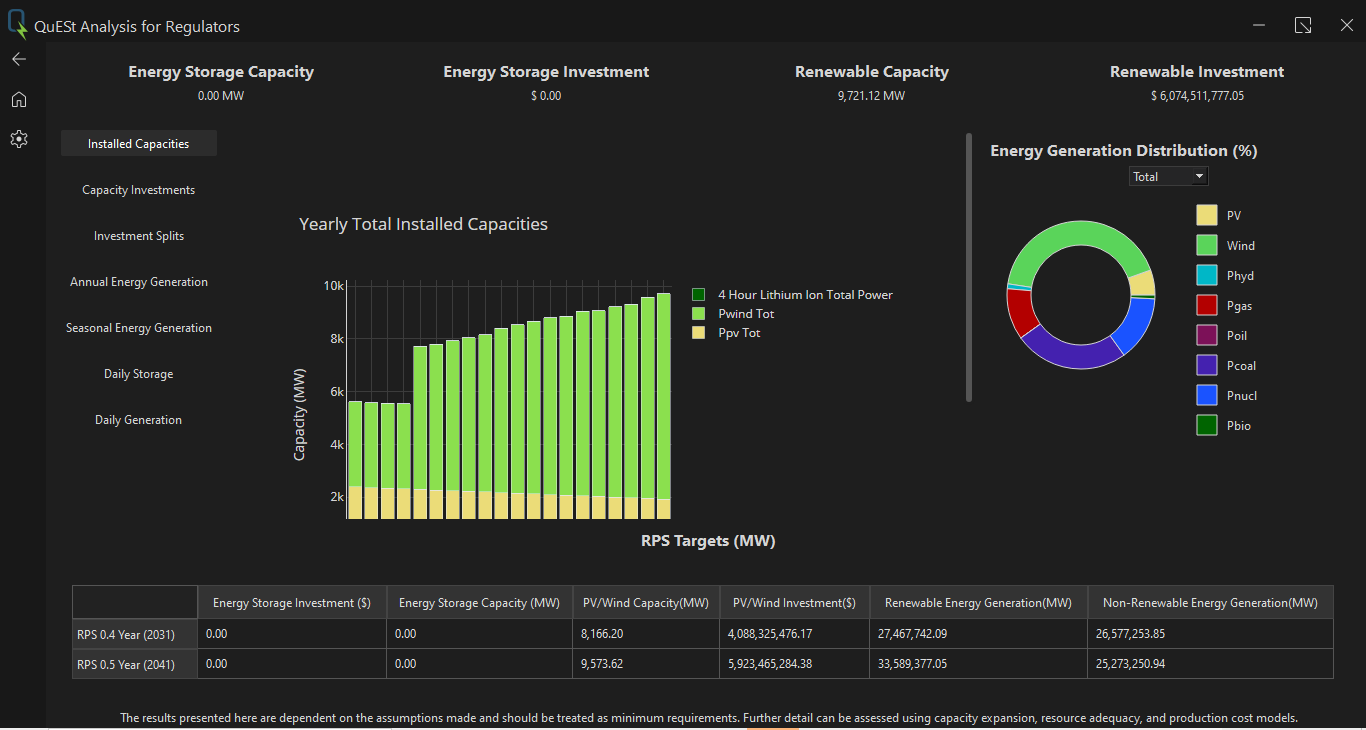
\includegraphics[width=0.8\textwidth]{pics/results_1.PNG}
\end{center}
The first image above shows results for the first futures scenario which is the most conservative in terms of generation retirements. This is run with the icc\_load.csv and cap\_samples\_f1a.csv files. There is significant investment in wind this first scenario and 9,721.12 MW in renewable generation overall totalling \$ 6,074,511,777.05 to meet the RPS goals and generation retirement targets. 

\begin{center}
    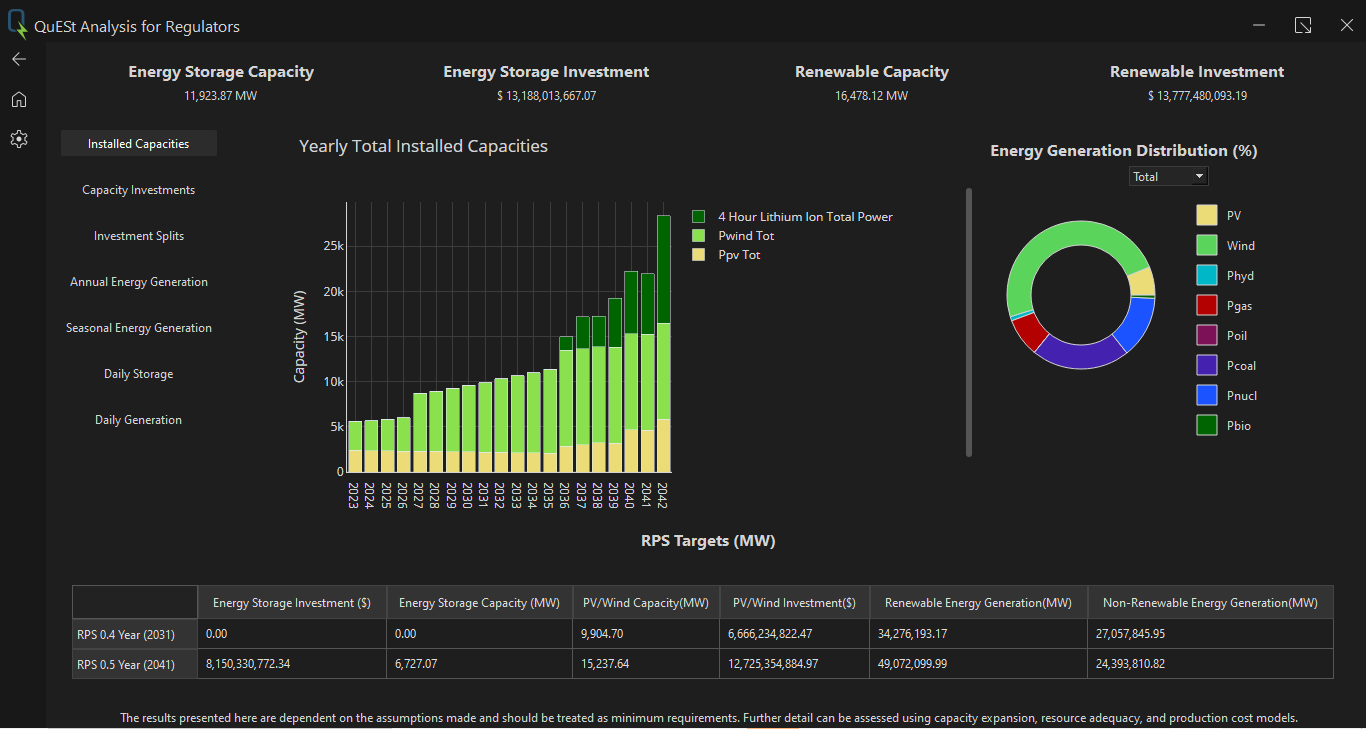
\includegraphics[width=0.8\textwidth]{pics/results_2.PNG}
\end{center}
The second image shows the results of running the second future scenario which is run with icc\_load2.csv and cap\_samples\_f2a.csv. Due to more generation retirement, this scenario requires more investment in renewables and the 4 hour lithium ion battery energy storage device with over \$13B invested in each. 

\begin{center}
    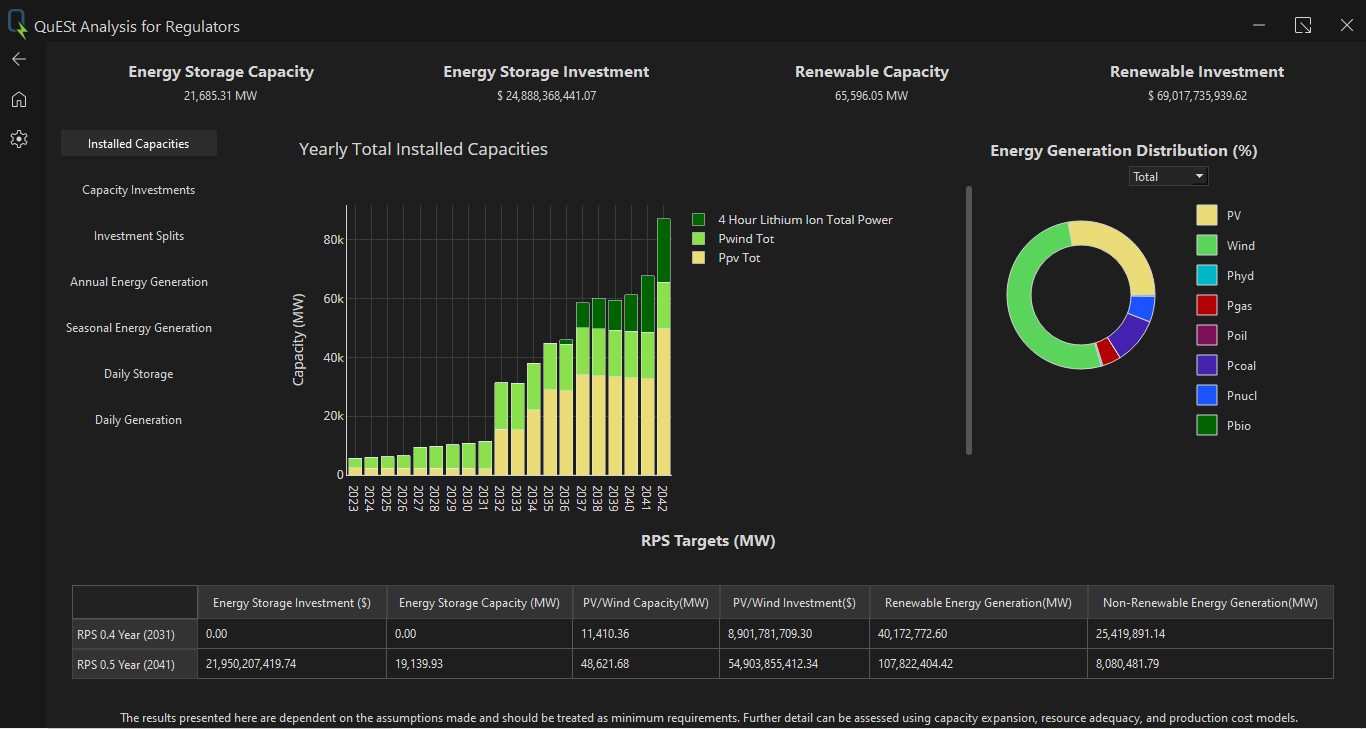
\includegraphics[width=0.8\textwidth]{pics/results_3.PNG}
\end{center}
The third image shows the results of running the third future scenario which is run with icc\_load3.csv and cap\_sammples\_f3a.csv. With the most extreme generation retirement the scenario requires the most investment requiring 21,385.31 MW of the 4 hour lithium ion battery at \$24.9B and 65,596.05 MW at \$69B. In all three cases the RPS target was not the driving factor in investments as the renewable generation exceeds the 50\% mark by 2031. These results should be taken as minimum requirements and more detailed analysis can be done with the QuESt Planning and PROGRESS tools.

\end{document}
